\documentclass[12pt]{article}\pagestyle{myheadings}

\title{Learning Chords Embeddings}
\author{Sephora Madjiheurem}
\usepackage[numbers]{natbib}
\usepackage{amsmath,amssymb,amsthm,amsfonts,graphics,subfigure,graphicx,enumerate,bbm} 

\newcommand{\R}{\mathbb{R}}
\newcommand{\C}{\mathbb{C}} 
\newcommand{\T}{\mathcal{T}}
\newcommand{\boldc}{\boldsymbol c}
\newcommand{\boldd}{\boldsymbol d}
\newcommand{\boldm}{\boldsymbol m}
\DeclareMathOperator*{\argmin}{argmin}


\begin{document}
\maketitle

\section{Linear Model}
\subsection{Skip-gram Model: Recap}

The skip-gram allows to efficiently learn high-quality distributed vector representations that capture precise syntactic and semantic word relationships \citep{mik2013}. We give here a short reminder of how the skip-gram model works. \\


We define a text as a sequence of words drawn from a finite vocabulary of size $W$. A word can be described as a ``one-hot'' vector $w_t \in \{0,1\}^W$, where exactly one entry is non-zero and the subscript $t$ represent the position of the word in the text.  
Given a  word $w_t$ in a text, define the context of word $w_t$ by $ C(w_t) = \{w_{t+j}, -m \leq j \leq m , j \neq 0\}$, where $m$ is the size of the context. We consider the conditional probability of a context given a word  $p(w_{t+j}|w_t)$.  The goal is to find word representations that are useful for predicting the surrounding words in a sentence. Formally, given a corpus of words of size $T$ and the context of word $w_t$ given by $C(w_t)$, the objective of the skip-gram model is to maximize the average log probability. 
\begin{equation}
\frac{1}{T} \sum_{t=1}^T \sum_{w \in C(w_t)} \log p(w|w_t)\,.
\label{eq:objective}
\end{equation}

The parametrization of the skip-gram model uses the architecture depicted in Figure~\ref{fig:skipgram} (from \citet{mik2013}). In this model, each output is computed using softmax to obtain the posterior distribution of context words:

\begin{equation}
p(w_{t+j}|w_t) = \frac{ \exp (v_{w_{t+j}}^T v_{w_t})}{\sum_{w=1}^W \exp (v_{w}^T v_{w_t})} \,\,,
\end{equation}

where $-m \leq j \leq m, j\neq 0$, $m$ is the size of the training context,  $v_w$ is the vector representation for $w$, and $W$ is the number of words in the vocabulary. \\

Detailed derivations and explanations of the parameter learning for this original skip-gram model can be found in \citep{Rong14}.

Because the computation cost of objective~(\ref{eq:objective}) is proportional to $W$ which can be very large when working with text training data, \citet{mik2013} use instead an efficient approximation, known as negative sampling (see \citep{NIPS2013_5021} for details). 

\begin{figure}[ht]
\centering
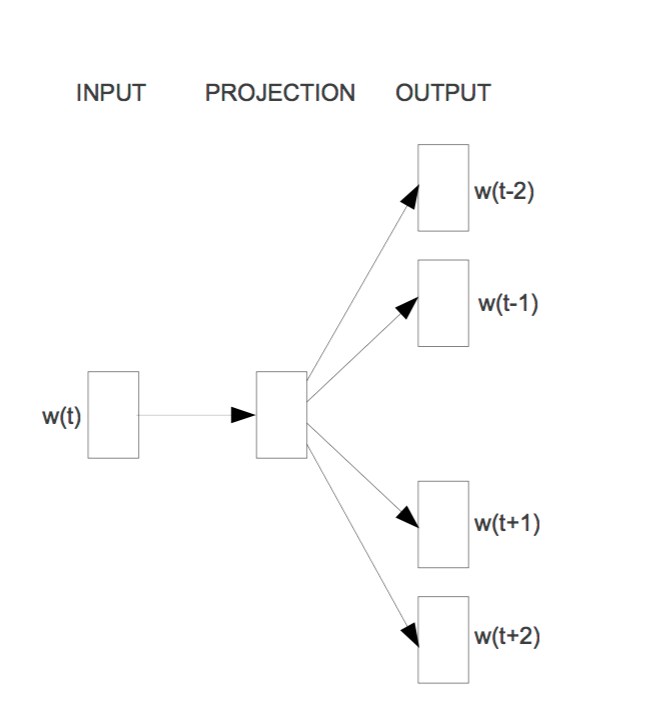
\includegraphics[width=.7\linewidth]{figures/skipgram.png}
\caption{\label{fig:skipgram}Skip-gram (\citet{mik2013})}
\end{figure}


\subsection{Chord2Vec}
Similarly to a text, we define a piece of music as a series of chords. A chord is a subset of notes drawn from a finite set of size $N$ and can be represented by a binary vector $\boldc = \{c_1, c_2, \ldots, c_N\}\in \{0,1\}^N$.\\

\noindent To adapt the skip-gram model to music data there are a few points that need to be considered:

\begin{enumerate}
\item A text can be represented as a sequence of words, where each word can be represented as a "one-hot" vector. In the case of music, we need a "many-hot" vector to represent a chord, as more than one note can be heard simultaneously.  
\item The set of notes is smaller than the vocabulary considered when working with text data.
\end{enumerate}
 

A naive adaptation is to use a separate sigmoid function at the output layer to predict each note in a chord. This makes the conditional independence assumption between the notes in a context chord $\boldc$ given a chord $\boldd$ , i.e \begin{equation}
p(\boldc | \boldd) = \prod_{n=1}^N  p(c_n |  \boldd) \,.
\end{equation} 

Using the weight matrix $M \in \R^{D \times N}$, we can compute a score for each note $c_i$ in a chord:

\begin{equation}
h(i,\boldd) = M_{(:,i)}^T \frac{M \boldd}{\mathbbm{1}^T \boldd} \,,
\end{equation}

where $M_{(:,i)}$ denotes the $i$'th row of $M$ and $\mathbbm{1}$ is the vector of all 1's of size $N$. 

\begin{equation}
p(c|d) = \prod_{n=1}^N \frac{1}{1 + \exp(-v_{c_{t+j}}^T v_{c_t})} \,\,\,,
\end{equation}

where $-m \leq j \leq m, j\neq 0$, $m$ is the size of the training context, $N$ is the number of different notes and  $v_c$ is the vector representation for chord $c$. \\

The second point, together with the fact that the computation of the objective is no longer dependent of number of possible context chords (since we are not using softmax, the sum over all possible context chords disappears) suggest that there might not be the need to use efficiency optimizations tricks as negative sampling. 
 
 
\section{Sequence autoencoding}
\subsection{Sequence-to-sequence: Recap} 
Sequence-to-sequence models allow to learn a mapping of input sequences of varying lengths to output sequences also of varying lengths \citep{SutskeverVL14}. It uses a neural network known as RNN Encoder-Decoder. Figure~\ref{fig:seq2seq} depicts the model architecture. 
\begin{figure}[ht]
\centering
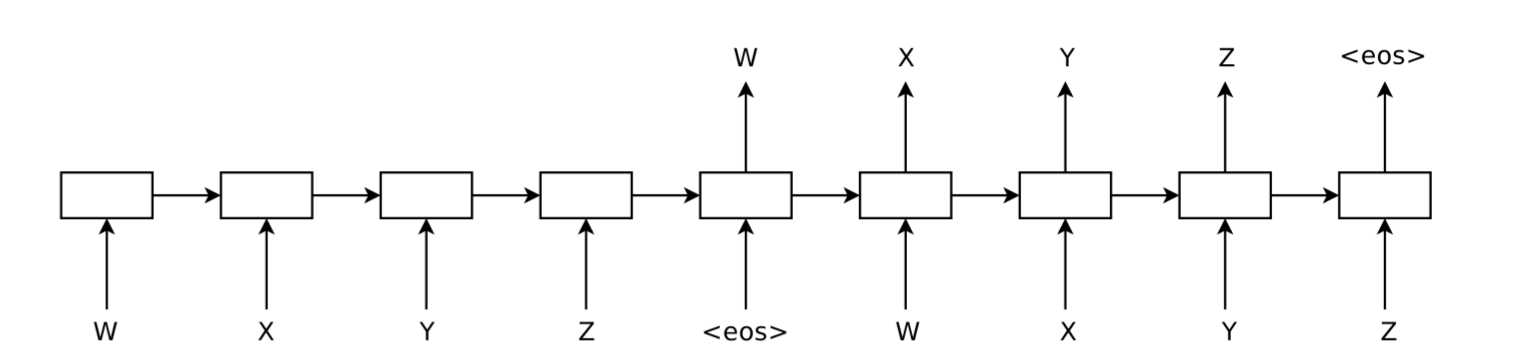
\includegraphics[width=1.0\linewidth]{figures/seq2seq.png}
\caption{\label{fig:seq2seq}Sequence-to-sequence (\citet{SutskeverVL14})}
\end{figure}
An LSTM encoder is used to map the input sequence to a fixed length vector, and another LSTM decoder is then used to extract the output sequence from this vector. The general goal is to estimate 
$
p(y_1,\ldots,y_{T'} | x_1, \ldots, x_T)\,,
$
where $x_1, \ldots, x_T$ and  $y_1,\ldots,y_{T'}$ are the input and output sequences respectively, and $T'$ and $T$ need not to be equal. 
\\

The objective is given by:

\begin{equation}
\max_{\theta} \frac{1}{|\T|} \sum_{(X,Y) \in \T} \log p(Y|X,\theta) \,,
\label{eq:seq2seq_obj}
\end{equation}

where $Y$ is a correct output given the input $X$ and $\T$ is the training set and $\theta$ is the set of the model parameters. 
The encoder and decoder are jointly trained to maximize the objective according to $\theta$.
\\

The model estimates the conditional probability $p(y_1,\ldots,y_{T'} | x_1, \ldots, x_T)$ by first obtaining the fixed-length vector representation $v$ of the input sequence (given by the last state of the LSTM encoder) and then computing the probability of $y_1,\ldots,y_{T'} $ with the LSTM decoder: 

\begin{equation}
p(y_1,\ldots,y_{T'} | x_1, \ldots, x_T) = \prod_{t=1}^{T'} p(y_t|v, y_1,\ldots,y_{t-1})
\end{equation}

\subsection{Chord-to-chord}
The sequence-to-sequence model can be used to learn embeddings for chords, by training the model to learn the context of a given chord. 

In this setting, a chord is represented as a sequence of notes in some fixed ordering: $c \subseteq N$, where $N$ is the ordered set of all possible notes. A chord can have an arbitrary size. 

The goal is then to estimate
$
p(n^{(j)}_1, \ldots, n^{(j)}_T | n_1,\ldots,n_{T'})\,,
$
where the $n$'s are in $N$, $ c_t=n_1,\ldots,n_{T'}$ is an input chord and $c_{t+j} =n^{(j)}_1, \ldots, n^{(j)}_T$ is the $j^{th}$ neighbor of $c$.

If $C(c_t)$ denotes the set of chords that are in the neighborhood of the chord $c_t$, then the objective in (\ref{eq:seq2seq_obj}) can be written as:

\begin{equation}
\max_{\theta}  \frac{1}{W} \sum_{t=1}^{W} \sum_{c\in C(c_t)} \log p(c|c_t,\theta)\,,
\label{eq:objective}
\end{equation}

Where $W$ is the size of the corpus of chords in the training data. 


\subsection{Chord-to-chords}
An alternative to estimating the probability of single context chord is to estimate the probability of the entire neighborhood 
$
p(C(c_t) | c_t)\,,
$
by combining all context chord in one longer output sequence. 

The corresponding objective is then given by:
\begin{equation}
\max_{\theta}  \frac{1}{W} \sum_{t=1}^{W} \log p(C(c_t)|c_t,\theta)\,,
\label{eq:objective}
\end{equation}


\newpage
\bibliographystyle{plainnat}
\bibliography{bibli.bib} 

\end{document}